\subsection{Trivial examples}

\begin{frame}
  \frametitle{Trivial examples}
  \begin{itemize}
  \item Located in the \texttt{examples/01\_trivial/} directory.
  \item Contains trivial examples, introducing the following concepts.
    \begin{itemize}
    \item Project files
    \item Console application basics
    \item GUI application basics
    \item Some of the Qt's utility classes
    \item Building projects with \texttt{qmake}.
    \end{itemize}
  \end{itemize}
\end{frame}

\subsection{Hello world - console}

\begin{frame}[fragile]
  \frametitle{Hello world -- console}
  Located in \texttt{examples/01\_trivial/01\_hello\_console/}:
  \begin{itemize}
  \item \texttt{main.cpp} -- the main and only source file
  \begin{lstlisting}[basicstyle=\scriptsize\ttfamily]
	#include <QTextStream>
 	 
	int main(void)
	{
	    QTextStream(stdout) << "Hello, console!" << endl;
	    return 0;
	}
  \end{lstlisting}
  \item \texttt{hello.pro} -- the Qt project file
  \begin{lstlisting}
	SOURCES += main.cpp
	TARGET   = hello_console
  \end{lstlisting}
  \end{itemize}
\end{frame}

\subsection{Hello world - GUI}

\begin{frame}[fragile]
  \frametitle{Hello world -- GUI}
  Located in \texttt{examples/01\_trivial/02\_hello\_gui/}:
  \begin{itemize}
  \item \texttt{main.cpp} -- the main source file
  \begin{lstlisting}[basicstyle=\scriptsize\ttfamily]
	#include <QtGui>
	#include <QApplication>
	#include <QLabel>

	int main(int argc, char* argv[])
	{
	    QApplication app(argc, argv);
	    QLabel label("<I>Hello</I>, <B>GUI</B> world!");
	    label.show();
	    return app.exec();
	}\end{lstlisting}
  \item \texttt{hello.pro} -- the project file
  \begin{lstlisting}
	(*@\alert{QT      += widgets}@*)
	SOURCES += main.cpp
	TARGET   = hello_gui
  \end{lstlisting}
  \end{itemize}
\end{frame}

\subsection{Hello world - XML-UI}

\begin{frame}
  \frametitle{Hello world -- XML-UI}
  Located in \texttt{examples/01\_trivial/03\_hello\_xml\_ui/}:

  \begin{itemize}
  \item \texttt{mainwindow.ui} -- an external XML file defining the form layout.
  \item \texttt{mainwindow.h} -- C++ header declaring the \texttt{MainWindow} class.
  \item \texttt{mainwindow.cpp} -- C++ file implementing the \texttt{MainWindow} class.
  \item \texttt{main.cpp} -- C++ file implementing the \texttt{main} function.
  \item \texttt{hello.pro} -- The Qt project file.
  \end{itemize}
\end{frame}

\begin{frame}[fragile]
  \frametitle{Hello world -- XML-UI}
  File \texttt{mainwindow.ui}

\begin{lstlisting}[basicstyle=\tiny\ttfamily,language=XML]
<?xml version="1.0" encoding="UTF-8"?>
<ui version="4.0">
 <class>MainWindow</class>
 <widget class="QMainWindow" name="MainWindow">
  <property name="geometry">
   <rect>
    <x>0</x><y>0</y><width>200</width><height>100</height>
   </rect>
  </property>
  <property name="windowTitle"><string>Hello</string></property>
  <widget class="QWidget" name="centralWidget">
   <widget class="QLabel" name="label">
    <property name="geometry">
     <rect>
      <x>40</x><y>40</y><width>120</width><height>20</height>
     </rect>
    </property>
    <property name="text">
     <string>&lt;I&gt;Hello&lt;/I&gt;, &lt;B&gt;GUI&lt;/B&gt; World!</string>
    </property>
    <property name="alignment"><set>Qt::AlignCenter</set></property>
   </widget>
  </widget>
 </widget>
</ui>
\end{lstlisting}
\end{frame}

\begin{frame}[fragile]
  File \texttt{mainwindow.h}

  \begin{lstlisting}[basicstyle=\scriptsize\ttfamily]
	#ifndef MAINWINDOW_H
	#define MAINWINDOW_H

	#include <QMainWindow>

	namespace Ui { class MainWindow; }

	class MainWindow
 	 : public QMainWindow
	{
	    Q_OBJECT
	public:
	    explicit MainWindow(QWidget *parent = 0);
	    ~MainWindow();
	private:
	    Ui::MainWindow *ui;
	};

	#endif // MAINWINDOW_H
  \end{lstlisting}
\end{frame}


\begin{frame}[fragile]
  File \texttt{mainwindow.cpp}

  \begin{lstlisting}
	#include "mainwindow.h"
	#include "ui_mainwindow.h"

	MainWindow::MainWindow(QWidget *parent)
 	 : QMainWindow(parent)
 	 , ui(new Ui::MainWindow)
	{
	    ui->setupUi(this);
	}

	MainWindow::~MainWindow()
	{
	    delete ui;
	}
  \end{lstlisting}
\end{frame}


\begin{frame}[fragile]
  File \texttt{main.cpp}

  \begin{lstlisting}
	#include "mainwindow.h"
	#include <QApplication>

	int main(int argc, char *argv[])
	{
	    QApplication a(argc, argv);
	    MainWindow w;
	    w.show();

	    return a.exec();
	}
  \end{lstlisting}
\end{frame}


\begin{frame}[fragile]
  File \texttt{hello.pro}

  \begin{lstlisting}
	TEMPLATE  = app
	QT       += core gui widgets
	TARGET    = hello_xml_ui

	SOURCES  += main.cpp mainwindow.cpp
	HEADERS  += mainwindow.h
	FORMS    += mainwindow.ui
  \end{lstlisting}

  \begin{itemize}
  \item Output:
    \begin{figure}[!t]
    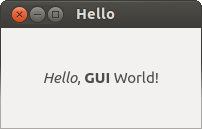
\includegraphics[width=0.3\textwidth]{images/hello_gui.png}
    \end{figure}
  \end{itemize}

\end{frame}


\begin{frame}[fragile]
  \frametitle{Hello world -- QML}
  Located in \texttt{examples/01\_trivial/04\_hello\_qml/}:

  File \texttt{hello.qml}

  \begin{lstlisting}[basicstyle=\tiny\ttfamily]
	import QtQuick 2.0
	import QtQuick.Window 2.0

	Window {
	    width: 320; height: 130
	    color: "lightgreen"

	    Text {
	        text: "Hello QML world!"
	        y: 40
	        anchors.horizontalCenter: parent.horizontalCenter
	        font.pointSize: 24
	        font.bold: true
	    }
	    Text {
	        text: "Click to close"
	        y: 80
	        anchors.horizontalCenter: parent.horizontalCenter
	        font.pointSize: 12

	        MouseArea {
	            anchors.fill: parent
	            onClicked: Qt.quit()
	        }
	    }
}
  \end{lstlisting}

\end{frame}

\begin{frame}[fragile]
  \frametitle{Hello world -- QML}

  \begin{itemize}
  \item Running the example:
  \begin{itemize}
    \item \verb@$> qmlscene hello.qml@
  \end{itemize}
  \item Output:
    \begin{figure}[!t]
    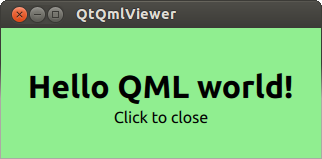
\includegraphics[width=0.4\textwidth]{images/hello_qml.png}
    \end{figure}
  \end{itemize}
\end{frame}

